\documentclass[a4paper,10pt]{jsarticle}

% レイアウト
\setlength{\textwidth}{\fullwidth}
\setlength{\textheight}{39\baselineskip}
\addtolength{\textheight}{\topskip}
\setlength{\voffset}{-0.5in}
\setlength{\headsep}{0.3in}
\pagestyle{myheadings}

% パッケージ
\usepackage[dvipdfmx]{graphicx}
\usepackage{amsmath,amssymb,epsfig}
\usepackage{bm}
\usepackage{ascmac}
\usepackage{pifont}
\usepackage{multirow}
\usepackage{enumerate}
\usepackage{cases}
\usepackage{type1cm}
\usepackage{cancel}
\usepackage{url}
\usepackage[dvipdfmx]{color}
\usepackage{listings,jlisting}
% 大きな中括弧
\usepackage{cases}

% 定義
\DeclareMathOperator*{\argmin}{arg\,min}
\DeclareMathOperator*{\argmax}{arg\,max}
\def\vec#1{\mbox{\boldmath$#1$}}
\def\R{{\Bbb R}}

% カウンタの設定
\setcounter{section}{0}
\setcounter{subsection}{0}
\setcounter{subsubsection}{0}
\setcounter{equation}{0}

% キャプションの図をFigに変更
\renewcommand{\figurename}{Fig.}
\renewcommand{\tablename}{Tab.}

% 式番号を式(章番号.番号)に
% \makeatletter
% \renewcommand{\theequation}{\arabic{section}.\arabic{equation}}
% \@addtoreset{equation}{section}
% \makeatother

% プログラムに色をつける
\usepackage{color}

\definecolor{codegreen}{rgb}{0,0.6,0}
\definecolor{codegray}{rgb}{0.5,0.5,0.5}
\definecolor{codepurple}{rgb}{0.58,0,0.82}
\definecolor{backcolour}{rgb}{0.95,0.95,0.92}

\lstdefinestyle{mystyle}{
    backgroundcolor=\color{backcolour},
    commentstyle=\color{codegreen},
    keywordstyle=\color{magenta},
    numberstyle=\tiny\color{codegray},
    stringstyle=\color{codepurple},
    basicstyle=\footnotesize,
    breakatwhitespace=false,
    breaklines=true,
    captionpos=b,
    keepspaces=true,
    numbers=left,
    numbersep=5pt,
    showspaces=false,
    showstringspaces=false,
    showtabs=false,
    tabsize=2
}

\lstset{style=mystyle}

% 表紙
\title{知能システム学特論レポート}
\author{
(DL2班)Caffe on Ubuntu\\
}
\date{2015年\ 7月\ 27日}

% ドキュメントの開始
\begin{document}
\maketitle
\section{報告者}
\begin{list}{}{}
 \item 15344203\hspace{0.5cm} 有田 裕太
 \item 15344206\hspace{0.5cm} 緒形 裕太
 \item 15344209\hspace{0.5cm} 株丹 亮
 \item 12104125\hspace{0.5cm} 宮本 和
\end{list}

\section{進行状況}

\begin{itemize}
\item ドロップアウトの理論について
\item Caffeを用いてドロップアウトを試してみた
\item データセットを増やした,学習パラメータの調整
\end{itemize}

\section{理論研究}

%%%%%% ogata %%%%%%
\subsection{誤差関数}
本班のcaffeを用いた画像分類では,第4回レポートで記したような多クラス分
類を行っており,出力関数はソフトマックス関数である.多クラス分類ではネッ
トワークが実現する関数を各クラスの事後確率のモデルであると見なし,そのモ
デルのもとで訓練データに対するネットワークパラメータの尤度を評価し,これ
を最大化する.いま訓練データとして,入力${\bf x}$とその正解クラスの組$C_k$が与え
られたとする.このときの目標出力の
2値の値を$K$個並べたベクトル${\bf
d}_n$によって表現すると,事後分布は次式のようになる.

\begin{equation}
 p({\bf d}|{\bf x}) = \prod_{k=1}^{K}p(C_k|{\bf x})^{d_k}
\end{equation}

これより,訓練データ${({\bf x}_n|{\bf d}_n)}(n=1,...,N)$に対する{\bf w}
の尤度は

\begin{equation}
 L({\bf w})=\prod_{n=1}^{N}p({\bf x}_n|{\bf x}_n;{\bf
	w})=\prod_{n=1}^{N}\prod_{k=1}^{K}p(C_k|{\bf
	x})^{d_{nk}}=\prod_{n=1}^{N}\prod_{k=1}^{K}(y_k({\bf x};{\bf w}))^{d_{nk}}
\end{equation}

と導ける.この尤度の対数とって符号を反転した次の式を誤差関数として用いる.
この関数は交差エントロピー(cross entropy)と呼ばれる.
\begin{eqnarray}
 E({\bf w})=-\sum^{N}_{n=1}\sum^{N}_{k=1}d_{nk}\log
	y_{k}(\vec{x}_{n};{\bf w})
\end{eqnarray}


\section{プログラミング}
\subsection{Caffeのドロップアウトを試す}
今まではアニメーション(ラブライブ!)を切り出して学習を行って,性能評価を行った.
そこで実在する人物の識別を行うためのデータセットとして,韓国の女性アイドルグループ(少女時代)のメンバーの識別を試みた.
アニメのキャラクター識別では学習の結果を解析したが良好な精度で学習ができ,過学習の傾向は見られなかった.
しかし少女時代のメンバーのクラスタリングでは用いたデータセットがアニメキャラクターの識別と比較して髪の色,光の当たり方,顔の向き等の条件が一定になりづらく学習の精度も低い.
このときの精度に関する結果をFig.~\ref{fig:過学習の傾向}に示す.
ただしこの結果はアニメキャラクターの学習でも同様に用いたCifar10のモデルで行っている.
Fig.~\ref{fig:過学習の傾向}より過学習の傾向が見られ,訓練データに関しての精度は$1$に収束しているが,テストデータに関しては精度は$77\%$程度である.

\begin{figure}[tb]
  \begin{center}
    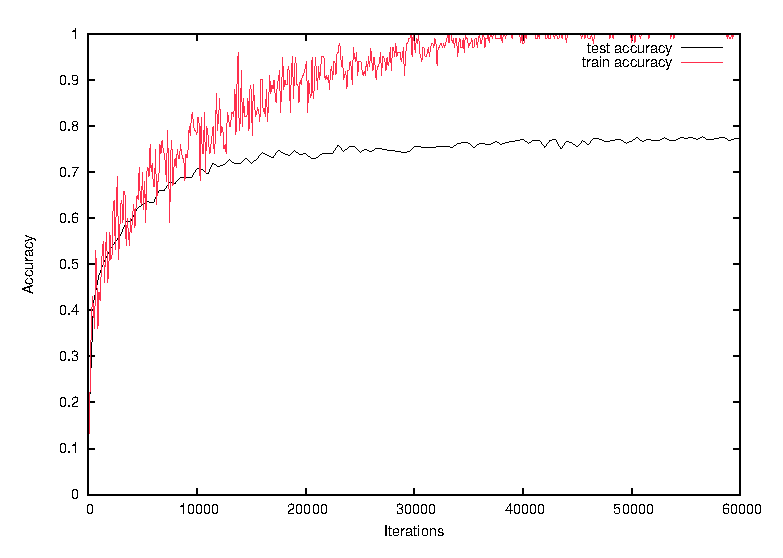
\includegraphics[clip,width=12cm]{./fig/eps/overtraining.eps}
  \end{center}
  \caption{過学習の傾向}
  \label{fig:過学習の傾向}
\end{figure}

したがって前節で説明したドロップアウトを導入し,過学習の回避を試みる.
ドロップアウトのユニットを追加するだけでなく,過学習が起きる原因となる学習データの不足が考えられるため単純にデータセットを増やす以外の方法で改善を行った.
その改善方法は入力として使うデータセットをランダムにクロップし入力データとして学習を行う方法と,入力データをランダムで左右反転させる方法である.
これらの工夫によって得られた結果をFig.~\ref{fig:ドロップアウトを追加し,データセットを増やす工夫を行った結果}に示す.
Fig.~\ref{fig:ドロップアウトを追加し,データセットを増やす工夫を行った結果}より訓練データにおける精度とテストデータにおける精度の乖離がなくなり過学習を抑えることができている.
また最終的なテストデータに関する精度は$88\%$と通常のCifar10のモデルを使用した場合よりも精度向上が見られた.

\begin{figure}[tb]
  \begin{center}
    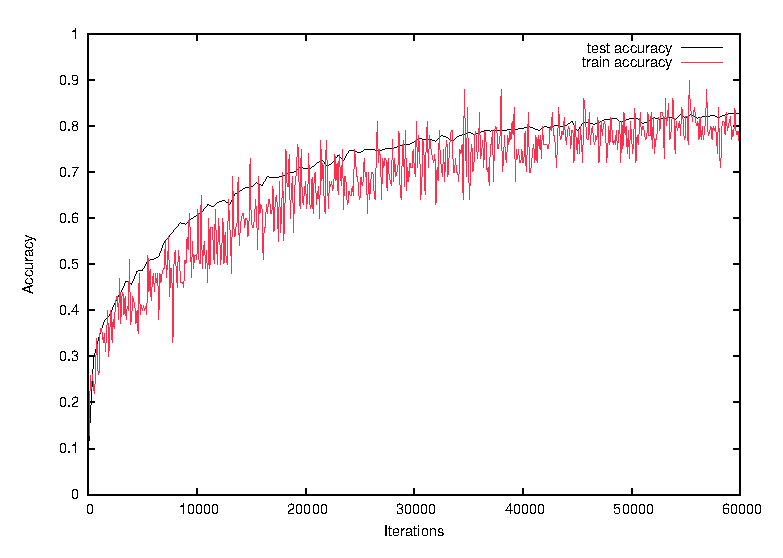
\includegraphics[clip,width=12cm]{./fig/eps/dropout.eps}
  \end{center}
  \caption{ドロップアウトを追加し,データセットを増やす工夫を行った結果}
  \label{fig:ドロップアウトを追加し,データセットを増やす工夫を行った結果}
\end{figure}

\subsection{データセットの強化}

アニメキャラクター(ラブライブ!)の識別で制度改善のためにデータセットを増やして再度学習を行った.また,学習の繰り返し回数も増やした.

前回と同様に従来のニューラルネットワークを用いて簡易的にクラスタリングを行った後,手動で修正を行った.その結果,各キャラクターに1000枚程度データセットを追加した.したがって,合計で9名のキャラクターそれぞれに約3000枚の画像を用意した.

学習を行った結果をFig.\ref{181752_26Jul15}に示す.Test Accuracyは最終的に$95.04\%$となった.
\begin{figure}[tb]
  \begin{center}
    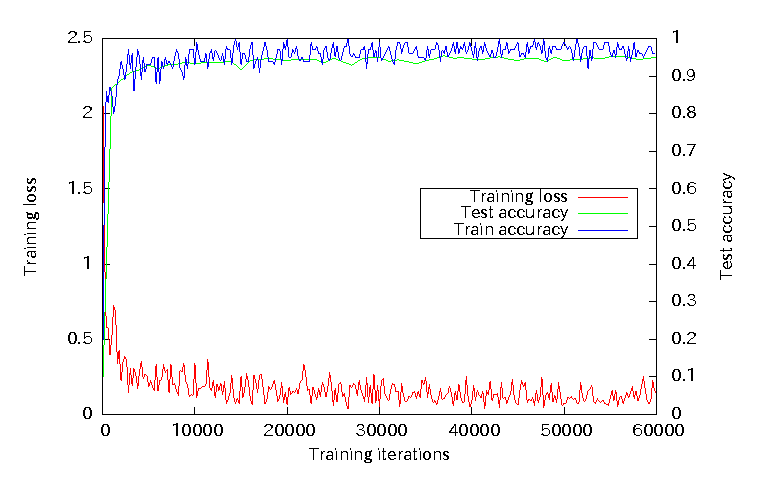
\includegraphics[clip,width=12cm]{./fig/eps/result_train_test_lovelive_full.eps}
  \end{center}
  \caption{データセットを増やして学習を行った結果}
  \label{181752_26Jul15}
\end{figure}


今回作成した識別器を使った識別結果と前回の識別結果をFig.とFig.に示す.誤認識が改善したことが分かる.

% \section{今後の課題}
% \begin{itemize}
%  \item 理論研究を進める.
%  \item 作成した識別器でどのような特徴量が利用されているのかを調査する.
% \end{itemize}

\end{document}